% < 1 https://quarkus.io
% < 1 https://books.google.at/books?hl=de&lr=&id=AH_EDwAAQBAJ&oi=fnd&pg=PP1&dq=quarkus&ots=ZJfLHasMm9&sig=K7__BsdmoksvoLfJSrqqGOPac1Y&redir_esc=y#v=onepage&q=quarkus&f=false
 
Quarkus wurde kreiert, um Applikationen zu erstellen, welche in einer modernen, cloud-nativen Welt funktionieren sollen. Quarkus ist ein kubernetes-natives Java-Framework, auf GraalVM und HotSpot zugeschnitten. Das Ziel von Quarkus ist es, JAVA zur führenden Plattform für Kubernetes und serverlose Umgebungen zu machen. Quarkus ist Open Source. \cite{quarkusOfficialSite}
 
Die größte Challenge von Mikroservicearchitekturen ist, dass die Vermehrung von Services die Komplexität des Systems erhöht. Diese kann mithilfe von Kubernetes-basierenden orchestrierenden Systemen1 gelöst werden, da somit die Effizienz sowie die Ressourcenverwertung erweitert werden können. Die Systeme regeln die zeitliche Planung und das Management der Mikroservices in einer dynamischen Weise. Dadurch kann man auch je nach Bedarf an dem System arbeiten, ohne dass die Gefahr besteht, dass ein Container ausfällt. Um nun die gesamten Komponenten zusammenzufügen, wurde das Framework Quarkus entwickelt.
 
Quarkus funktioniert ausgezeichnet, wenn es darum geht, Cloud-Native Applikationen von Unternehmen zu managen. Es ist in der Lage kurzen nativen Code aus Java Klassen zu bauen, sowie Container Images daraus zu erstellen. Diese Container können darauffolgend auf Kubernetes laufen. Außerdem unterstützt Quarkus die bekanntesten Java Libraries wie etwa RESTEasy, Hibernate, Apache Kafka, Vert.x, usw.
 
Wie nun schon vorher erwähnt, ist eines der vielversprechendsten Features von Quarkus die Fähigkeit aus Applikationen automatisch Container Images zu generieren. Durch das Generieren von Container Images aus nativen Applikationen wird außerdem eine Gefahr zunichte gemacht. Diese hat mit der nativen Ausführung des Programms zu tun, es handelt sich dabei um potentielle Konfliktfehler von Errors, wenn der Build auf einem anderen Operating System stattfand.
Quarkus sorgt außerdem dafür, imperative und reaktive Modelle zu verbinden. Reaktives Programmieren wird immer beliebter aus dem Grund, dass es in der Lage ist asynchrones Programmieren mit Daten Streams und der Veränderung von Daten zu verbinden. \cite{QuarkusBuch}
 
\subsection{Architektur}
Im Zentrum von Quarkus liegt die Kern Komponente, welche die Aufgabe hat, die Applikation in der Build-Phase umzuschreiben, um sie perfekt zu optimieren \ref{fig:impl:QuarkusArchitektur}. Daraus entsteht eine native ausführbare und Java-runnable Applikation. Damit der Quarkus-Kern diese Arbeit erledigen kann, müssen einige verschiedene Komponenten zusammenarbeiten:
 
\begin{compactitem}
    \item Jandex: Ein platzsparender Java Annotation Indexer, sowie eine offline Reflexions Library. Diese Bibliothek ist in der Lage alle runtime sichtbaren Java Annotationen und Klassenhierarchien für ein Set von Klassen in einer speichereffizienten Repräsentation zu indexen.    
    \item Gizmo: Gizmo ist eine Bytecode-Generations-Library, welche von Quarkus verwendet wird, um Java Bytecode zu produzieren.             
    \item GraalVM: Ein Set von Komponenten, in welchem jede eine bestimmte Funktion hat. Beispiele dafür sind: ein Compiler, ein SDK API für die Integration von Graal Sprachen und der Konfiguration von native images, runtime Umgebung für JVM-basierte Sprachen
    \item SubstrateVM: Unterkomponente von GraalVM, welche die ahead-of-time (AOT) Kompilation von Java Applikationen von Java Programmen zu eigenständigen ausführbaren Programmen erlaubt.
\end{compactitem}
 
Des Weiteren gibt es noch einige Quarkus Extensions. Dazu gehören die MicroProfile Spezifikationen, sowie ein Set von Extensions für Hibernate ORM, ein Transaktionsmanager (Narayana), ein Verbindungs-Pool-Manager und viele mehr. \cite{QuarkusBuch}
 
\begin{figure}
    \centering
    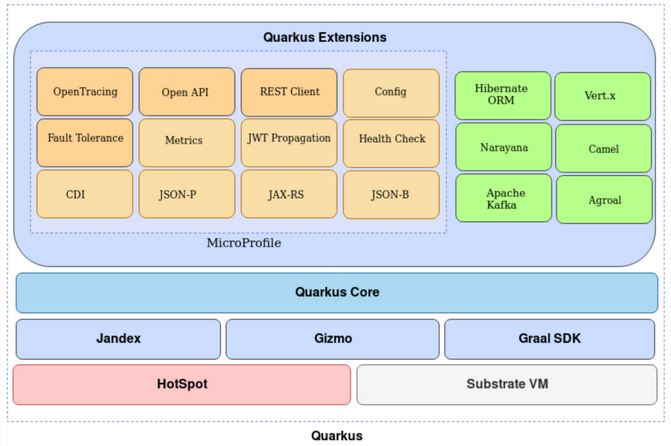
\includegraphics[scale=0.9]{pics/quarkusArchitektur.JPG}
    \caption{Quarkus Architektur \cite{QuarkusBuch}}
    \label{fig:impl:QuarkusArchitektur}
\end{figure}
 
\subsection{Funktionen}
\subsection{Vergleich zu anderen Tools}
% < https://devm.io/java/micronaut-speed-test-170870-001
% < https://micronaut.io/2020/04/07/micronaut-vs-quarkus-vs-spring-boot-performance-on-jdk-14/
Drei sehr vergleichbare Frameworks sind Quarkus, Micronout und Spring Boot. Sie besitzen alle ähnliche Features und Fähigkeiten.
Am wichtigsten ist dabei, welches Framework ist am schnellsten, welches am performantesten, welches benötigt den wenigsten Speicher.
\cite{Micr/QuarBenchmark}
 
\begin{compactitem}
    \item[Quarkus]
    \item Kubernetes-native, für Java designed, für GraalVM und OpenJDK Hotspot, besitzt die besten Java-Bibliotheken und Standards, schnell beim Starten
    \item[Micronout]
    \item Cloud-native, JVM-basiert, full-stack Framework für Mikro-Services und serverlose Anwendungen, geringer Speicherverbrauch
    \item[Spring Boot]
    \item Open-Source Java Framework, einfach um Stand-alone Anwendungen und Mikroservices zu kreieren, benötigt sehr wenig Konfiguration, um starten zu können
\end{compactitem}
\cite{Micr/QuarBenchmark}
 
Für einen näheren Vergleich zwischen den Frameworks, siehe \ref{fig:impl:Quarkusbenchmark}. Dabei kann erkannt werden, dass Quarkus Response Zeit die bestbewertete ist, Spring trotzt dabei mit einer Compilation Zeit von nur 1.33s, wenn der Befehl \texttt{./mnv clean compile} verwendet wird. Insgesamt kann allerdings aus dem Benchmark Vergleich gezogen werden, dass Micronout in den meisten Kategorien als Sieger hervorgeht. Vor allem, wenn einem ein kleiner Speicherverbrauch wichtig ist, sollte somit zu Micronout gegriffen werden. \cite{MicrVSQuarVSSprin}
 
\begin{figure}
    \centering
    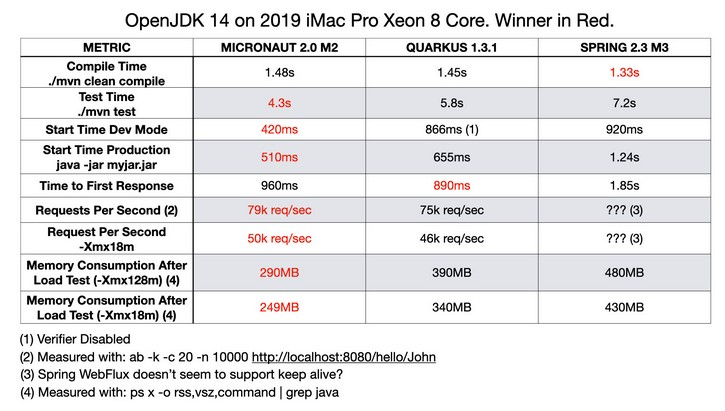
\includegraphics[scale=0.8]{pics/quarkus_benchmark.jpg}
    \caption{Quarkus Benchmark Test \cite{MicrVSQuarVSSprin}}
    \label{fig:impl:Quarkusbenchmark}
\end{figure}
 
\subsection{NodeJS im Vergleich}
\subsection{http GET/POST/PUT Funktionen}
% < 1 https://quarkus.io/guides/rest-json
Mithilfe von GET/POST/PUT können Daten an einen Webserver geschickt werden, um diese später z.B. in einer Webapplikation nutzen zu können.
 
Um diese Annotations verwenden zu können, muss eine REST Ressource erstellt werden.
Bei dieser Ressource muss zuallererst ein Pfad definiert werden. Dieser gilt für alle darauffolgenden Funktionen in der Ressource Klasse.
 
Die Funktionen in der Klasse sind alle für verschiedene GET- bzw. POST-Requests mit verschiedenen Pfaden verantwortlich. Bei jedem von ihnen wird definiert, ob ein GET, POST oder PUT Request abgesetzt werden soll. In der darauffolgenden Zeile wird ein Pfad angegeben, welcher zusätzlich nach dem über der Klasse angegebenen Pfad verwendet wird. Als letztes Attribut wird definiert, je nachdem ob der Request etwas auslesen soll oder etwas anzeigen lassen soll, ein @Produces bzw. ein @Consumes. In diesen wird jeweils der Typ von dem auszulesenden bzw. anzuzeigenden angeführt. In dem Beispiel unterhalb ist es ein JSON-Format. \cite{quarkusRest}
\begin{lstlisting}[language=java,caption=Quarkus POST-Request,label=lst:impl:canvasJSchartOptions]
    @GET
    @Produces(MediaType.APPLICATION_JSON)
    @Path("/all/animal")
    public Set<Animal> getAll() {
        return animalRepository.getAll();
    }
  \end{lstlisting}


 
\subsection{JDBC und JPA}
% < 1 https://quarkus.io/guides/hibernate-orm
% < Java ist auch eine Insel, Christian Ullenboom, 2018 S1111-1121 

%  < https://books.google.at/books?hl=de&lr=&id=UHobxmgB714C&oi=fnd&pg=PR1&dq=jpa&ots=ijY_GdSJ5U&sig=IlRJxhMjrF4xF2-NXQ-OdM6f48Q&redir_esc=y#v=onepage&q=jpa&f=false, von  Mike Keith S5-16


\begin{compactitem}
    \item [JPA]
    \item JPA ist die Abkürzung für Jakarta Persistance API. Es ist eine POJO-basiertes Framework für Java Persistance. Die Hauptaufgabe von JPA ist dabei das objekt-relationale Mapping, allerdings bietet JPA auch eine Lösungen für die architektonische Herausforderung der Integrierung von Persistance an. 
    \item [JDBC]
    \item Um in Java auf eine relationale Tabelle Zugriff zu erhalten, wird JDBC benötigt. JDBC ist dabei eine Abkürzung für Java Database Connectivity. JDBC fasst einen Satz von Schnittstellen zusammen, welcher nötig ist, damit sich Java an relationale Datenbanken anbinden kann. Durch JDBC kann somit eine Verbindung zu einer Datenbank aufgebaut werden, auf Tabellen zugegriffen werden, Daten ausgelesen oder verändert werden.  
\end{compactitem}
\cite{quarkusHibernate}

\subsubsection{Quarkus und JDBC}
Um Quarkus im Verbindung mit Datenbanken verwenden zu können, mus ein passender JDBC-Driver verwendet werden. Dabei gibt es für jede Datenbank einen eigenen passenden Driver. Bei einer PostgreSQL-Datenbank, welche in diesem Projekt verwendet wurde, lautet die artifactId (welche in verwendet wird um den JDBC-Driver als Dependency einzubinden), \texttt{quarkus-jdbc-postgresql}. \ref{lst:impl:JDBCDependency} Diese Dependency muss in die pom.xml Datei des Programms kopiert werden. Bei starten des Projekts wird der JDBC-Driver anschließend automatisch hinzugefügt. \cite{quarkusHibernate}
\begin{lstlisting}[language=html,caption=JDBC Dependency,label=lst:impl:JDBCDependency]
    <dependency>
        <groupId>io.quarkus</groupId>
        <artifactId>quarkus-jdbc-postgresql</artifactId>
    </dependency>
  \end{lstlisting}

